\documentclass[12pt,fleqn]{article}\usepackage{../../common}
\begin{document}
Monte-Carlo Ağaç Araması (Monte Carlo Tree Search -MCTS-), Oyun Oynayan Yapay Zeka

Otomatik oyun oynayan yapay zeka öğreten derslerdeki kilometre taşlarından
biri altüst / minimaks algoritmasiydi. Notlarımızda anlattığımız bu
algoritma, bir oyunda bizim yaptığımız, rakibin yaptığı tüm hamle
seçeneklerine göre oluşan tahta konfigürasyonlarına bakarak ve bu tahtalara
değer atayabilen bir değer fonksiyonuyla onları irdeleyerek rakip için en
kötü bizim için en iyi olacak şekilde bir arama ile optimal oyun
hamlelerini buluyordu. 

Fakat minimaksın bir problemi şudur: birkaç hamle sonrasına bakmak için tüm
mümkün hamlelere göre kurulan ağaç müthiş büyük olabilir. Özellikle Go
oyunu [1] gibi dallanma faktörü çok büyük olan oyunlarda minimaks zorluk
yaşayabiliyor. Bu gibi durumlarda MCTS yaklaşımının daha başarılı olduğu
bulunmuştur. 

Şimdi MCTS'i anlatalım, özelde UCT adı verilen üst güven aralığının
ağaçlara uygulanması (upper-confidence applied to trees) adlı çeşidini
gösterelim. Bunun için tabii önce UCT'yi ve onun baz çeşidi UCB1'i anlamak
lazım.

Kumarhanelerdeki o kollu oyun makinalarını düşünelim, oyuncunun önünde
bunlardan birkaç tane olsun, ve bu makinalardan her birinin farklı ve
bilinmeyen bir getiri dağılımı var. Tek kollu makinalara argoda ``tek kollu
soyguncu (one-armed bandit)'' de denilir, bilgisayarcılar üstteki üstteki
probleme ``çok kollu soyguncu (multi-armed bandit)'' ismi veriyorlar. Biraz
esprili bir şekilde bu makinaları çok kollu bir ahtapotun hayal ediliyor
bazen, ki ahtapot akıllı, yani oyunu optimal oynayacak bilgisayar programı.

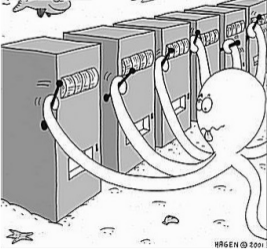
\includegraphics[width=13em]{mcts_01.png}

Aklımızdaki soru şu; Getirisi en iyi olacak makina acaba hangisi? Bilsek
hemen onu oynardık. Bunu başta bilmiyoruz, oturup başkasını seyredecek
durumda değiliz, o zaman hem seçenekleri bir şekilde deneyecek ama bu
sırada çok getiri kaybı yaşamayacak aynı zamanda uzun vadede kazançta
kalacak şekilde bu oyunu oynamak istiyoruz. UCB1 adlı bir strateji bunu
yapabiliyor, bu stratejiye göre her makina $i$ için bir istatistiki güven
aralığı yaratılır, 

$$ \overline{x}_i \pm \sqrt{\frac{2 \ln n}{n_i}} $$

$\overline{x}_i$: Makine $i$'nin ortalama getirisi

$n_i$: Makine $i$'nin kaç kere oynandığı

$n$: Tüm oyunlar (tüm makinelerde kaç kere oynandığı)

Ve stratejimiz her adımda üst sınırı en yüksek olan makinayı
oynamaktır. Bunu yaptıkça o makinanın gözlenen ortalaması kazanca / kayıba
göre kayacak, ve güven aralığı ufalacak (elimizde daha fazla veri var
çünkü, daha fazla veri daha fazla kesinlik demek), ve diğer makinaların
aralığı genişleyecek. Bir noktada başka bir makinanın üst sınırı o anda
oynadığımızı geçecek, o zaman biz bu öteki makinaya geçeceğiz. Uzun vadede
bu strateji optimal olarak sonuç vermektedir.

Türetmek için notasyonu biraz değiştirelim [3], $a$ bir aksiyon (ya da
makina seçimi), $Q(a) = E(r|a)$, bir aksiyon için ortalama getiri, $U_t(a)$
adım $t$'de bir aksiyonun üst sınırı, $\hat{Q}, \hat{U}$ kestirme değerler,
$N(a)$ bir aksiyonun kaç kez seçildiği. Hem $\hat{U}$ kestirme değerini
sürekli hesaplayacağız, hem de güven aralığını maksimize eden aksiyonu
seçeceğiz, yani.

$$ a_t = \arg \max_{a \in A} \hat{Q}_t(a) + \hat{U}_t(a) $$

Bu seçimi yaparken yüksek olasılıkla (with high probability)
$Q(a) \le \hat{Q}_t(a) + \hat{U}_t(a)$ olmasını sağlayacağız. Bu şart için
Hoeffding eşitsizliğinden başlayabiliriz (bkz [5]).

$X_1,...X_n$ $[0,1]$ aralığında bağımsız özdeşçe dağılmış (i.i.d.)
değerlere sahip rasgele değişkenler olsunlar, ve
$\overline{X}_t = \frac{1}{\tau} \sum_{\tau=1}^{t} X_\tau$ örneklem
ortalaması olsun. O zaman

$$ P(E(X) > \overline{X}_t + u ) \le e^{-2 t u^2}$$

olduğunu biliyoruz, soyguncu problemindeki getiri rasgele değişkenleri için
uyarlarsak,

$$ 
P \big( Q(a) > \hat{Q}_t(a) + U_t(a)  \big) \le 
e^{-2 N_t(a)U_t(a)^2 }
$$

İstediğimiz şartların oluşması için üstteki formülün doğruluğu yeterli,
şimdi bu formülü baz alarak bir $U_t(a)$ hesaplayabiliriz, formülü $U_t(a)$
tek başına kalacak şekilde tekrar düzenleyebiliriz. Eşitliğin sol tarafına
$p$ diyelim, burada sanki istenilen bir güven aralık büyüklüğünü baz almış
oluyoruz, 95\% (yani 0.95) gibi, ama burada sembolik bir değer kulladık,
ilk amacımız $u$ değerine erişmek,

$$ e^{-2 N_t(a)U_t(a)^2 } = p $$ 

$$ \ln p = -2 N_t(a)U_t(a)^2 $$

$$ \frac{-\ln p}{2 N_t(a)} = U_t(a)^2 $$

$$ U_t(a) = \sqrt{\frac{-\ln p}{2 N_t(a)}} $$

$t$ büyüdükçe $p$ azalsın istiyoruz, o zaman $p = t^{-4}$ seçebiliriz, bu
spesifik değer formülü de basitleştirmek için seçildi bir yandan,

$$ U_t(a) = \sqrt{\frac{\log t}{N_t(a)}} $$

Böylece UCB1 algoritmasına erişmiş olduk, 

$$ 
a_t = \arg \max_{a \in A} Q(a) + \sqrt{\frac{\log t}{N_t(a)}}
$$

UCT ve Tic-Tac-Toe

Oyunlar ve Monte Carlo işin için nasıl dahil oluyor? Mesela her adımda bir
sonraki en iyi adımı bulmak istiyoruz, MC ile bu geçişi simüle ederiz, yani
rasgele tahta hamlelerini deneyerek iyi olan bitişleri bulmaya
uğraşırız. Bu yöntemin bir kötü tarafı, minimaks durumunda olduğu gibi, çok
fazla hamle seçeneği olduğu zaman ortaya çıkar, rasgele seçim de,
tüm seçenekleri deneyen deterministik seçim gibi yetersiz kalabilir.

UCT burada bir çözüm olarak görülebilir. Fikir şu: verili bir tahta
konumundan atılacak bir adım ötesi bir çok-kollu soyguncu problemi olarak
görülebilir. 

İlk faz seçim fazıdır, başlangıç konumundan aşağı inmeye başlarız, ve eğer
baktığımız tüm düğümlerde çok-kollu soyguncu seçimi için gerekli
istatistikler var ise seçim UCB1 ile yapılır, ve devam edilir. Bu ta ki
üzerinde istatistik olmayan (yani hiç ziyaret edilmemiş) bir düğüme
gelinceye kadar devam eder. Eğer böyle bir düğüm(ler) var ise onlar
arasından rasgele seçim yapılır, böylece o düğüm ve altındakiler ziyaret
edilmiş olur ve kayıp / kazanç sonrası onların da artık istatistikleri olur
ve bir sonraki adımda onlar da UCB1 ile seçiliyor (ya da seçilmiyor)
olacaktır.

Örnek olarak bir Tic-Tac-Toe oyunu için bir örnek görelim. X ve O taşları
var, biz O için hesap yapıyoruz diyelim. A pozisyonunda (en üst) tüm alt
pozisyonlar hakkında istatistik var. Mesela 1/2 görüyoruz, bu o pozisyondan
iki kere geçilmiş bu geçişlerden birisi oyunun kazanılması ile bitmiş (bu
bir kazanç en sol alttaki bitiş). Şimdi bir A'dan bir kez daha geliyoruz,
UCB1 bize pozisyon B'ye git diyor, o seviyede en sağdaki düğüm için hiç
bilgi yok, o zaman rasgele olarak o seçiliyor, oradan tek seçenek var, ve O
kazanıyor. Böylece B pozisyonundaki istatistik 2/3 haline
geliyor. Başlangıçtan oyun bitişine kadar her gidiş simulasyonda bir döngü,
eğer 100 kere simüle et dersek bu döngü 100 kere döner.

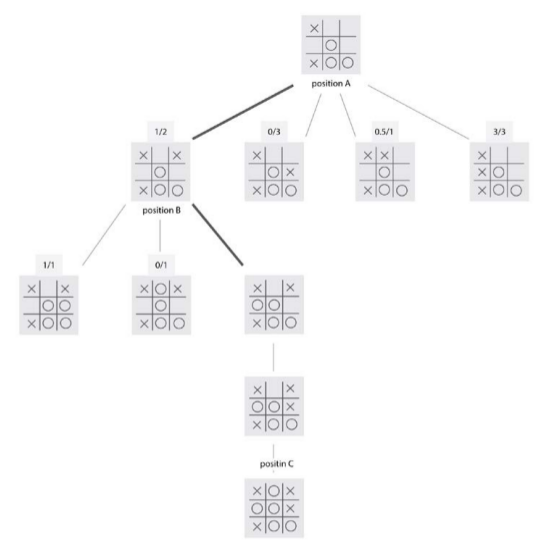
\includegraphics[width=30em]{mcts_02.png} 

Kod üzerinde görelim, üstteki başlangıç pozisyonundan X için (oyuncu 1,
öteki oyuncu -1) simulasyon yapalım, 1000 kere,

\inputminted[fontsize=\footnotesize]{python}{tictac_uct.py}

\begin{minted}[fontsize=\footnotesize]{python}
import tictac_uct
board_state = ((1, 0, 0),
               (0, -1, 0),
               (1, -1, -1))

res, move = tictac_uct.monte_carlo_tree_search_uct(board_state, 1, 1000)
print move
\end{minted}

\begin{verbatim}
(1, 0)
\end{verbatim}

X taşını üstten 2. satır ve 1. kolona koymamız isteniyor (Python 0 indisli
hatırlarsak), bu hareketi yapıyoruz,

\begin{minted}[fontsize=\footnotesize]{python}
b = np.array(board_state)
b[move] = 1.0
print b
\end{minted}

Ve bu kazanan hareket, resimde ikinci seviyede en sağdaki hamle
oluyor. UCB1 doğru tavsiyeyi vermiş gibi duruyor.

Not: MCTS algoritmasinin bol kullanım alanı var, A/B testlerinin
istatistiksel hesabı yerine MCTS kullanmak mümkün, yani iki sayfa versiyonu
arasında hangisinin daha iyi olduğu da bir tür çok-kollu soyguncu problemi
olarak görülebiliyor. 


Kaynaklar

[1] Bayramli, 
   {\em Go Oyunu, GnuGo}, 
   \url{https://burakbayramli.github.io/dersblog/sk/2018/02/go-gnugo.html}

[2] Bradberry, {\em Introduction to Monte Carlo Tree Search}, 
    \url{https://jeffbradberry.com/posts/2015/09/intro-to-monte-carlo-tree-search}

[3] Silver, {\em Reinforcement Learning}, 
    \url{http://www0.cs.ucl.ac.uk/staff/d.silver/web/Teaching.html}

[4] Zocca, {\em Python Deep Learning}

[5] Bayramli, İstatistik, {\em Ekler}

\end{document}
